\documentclass[12pt]{article}
\usepackage{amsfonts, amssymb, amsmath, amsthm}
\usepackage[margin=1in]{geometry}
\usepackage{tikz}
\usetikzlibrary{patterns, decorations.pathreplacing}

\pagestyle{myheadings}
\markright{Explainer: Rudin 2.22 — Separable Metric Spaces\hfill}

\newcommand{\R}{\mathbb{R}}
\newcommand{\Q}{\mathbb{Q}}
\newcommand{\N}{\mathbb{N}}

\begin{document}

\begin{center}
    \textbf{\Large Understanding Separable Metric Spaces}\\[0.5em]
    \large A visual guide to Rudin 2.22
\end{center}

\section{What Does ``Separable'' Mean?}

A metric space is \textbf{separable} if it contains a \textbf{countable dense subset}.

Let's break this down:

\begin{center}
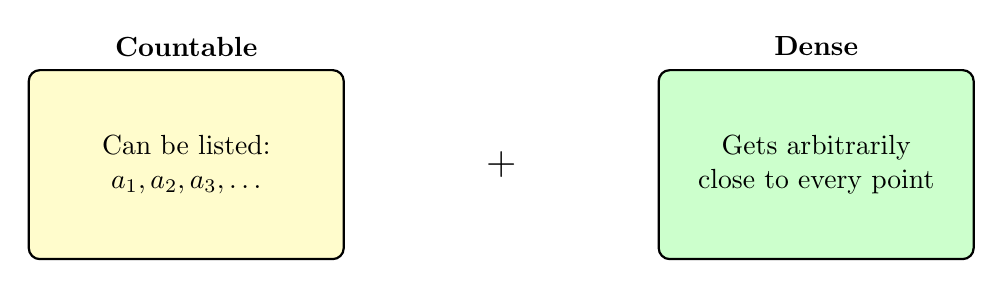
\begin{tikzpicture}[scale=1]
    % Countable
    \begin{scope}[xshift=-4cm]
        \draw[thick, rounded corners, fill=yellow!20] (-2, -1.2) rectangle (2, 1.2);
        \node at (0, 1.5) {\textbf{Countable}};
        \node[text width=3.5cm, align=center] at (0, 0) {Can be listed:\\$a_1, a_2, a_3, \ldots$};
    \end{scope}

    % Dense
    \begin{scope}[xshift=4cm]
        \draw[thick, rounded corners, fill=green!20] (-2, -1.2) rectangle (2, 1.2);
        \node at (0, 1.5) {\textbf{Dense}};
        \node[text width=3.5cm, align=center] at (0, 0) {Gets arbitrarily\\close to every point};
    \end{scope}

    % Plus sign
    \node at (0, 0) {\Large $+$};
\end{tikzpicture}
\end{center}

\section{What Does ``Dense'' Mean?}

A set $S$ is \textbf{dense} in $X$ if $\bar{S} = X$.

Equivalently: Every nonempty open set contains a point of $S$.

\begin{center}
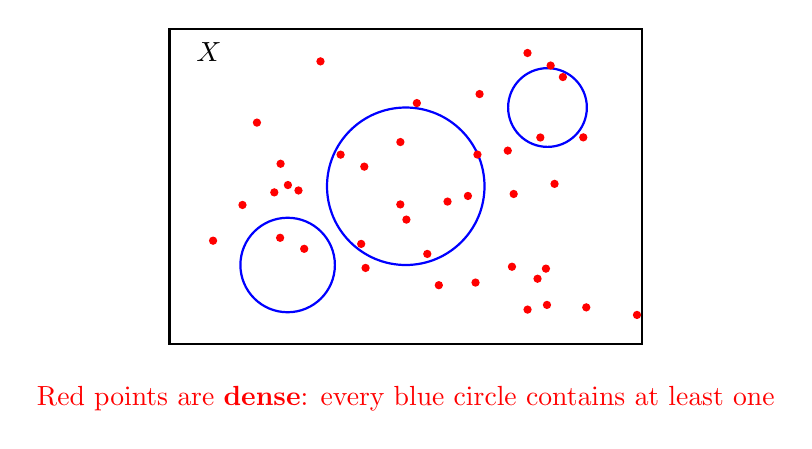
\begin{tikzpicture}[scale=1]
    % The space X
    \draw[thick] (-3, -2) rectangle (3, 2);
    \node at (-2.5, 1.7) {$X$};

    % Some open sets
    \draw[blue, thick] (0, 0) circle (1);
    \draw[blue, thick] (-1.5, -1) circle (0.6);
    \draw[blue, thick] (1.8, 1) circle (0.5);

    % Dense points (many dots)
    \foreach \i in {1,...,40} {
        \pgfmathsetmacro{\x}{-2.5 + 5.5*rnd}
        \pgfmathsetmacro{\y}{-1.7 + 3.4*rnd}
        \fill[red] (\x, \y) circle (1.5pt);
    }

    \node[red] at (0, -2.7) {Red points are \textbf{dense}: every blue circle contains at least one};
\end{tikzpicture}
\end{center}

\section{The Classic Example: $\Q$ is Dense in $\R$}

Between any two real numbers, there's a rational number.

\begin{center}
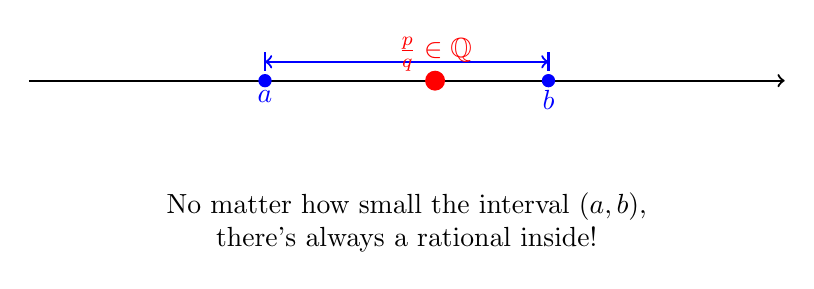
\begin{tikzpicture}[scale=1.2]
    % Number line
    \draw[thick, ->] (-4, 0) -- (4, 0);

    % Two reals
    \fill[blue] (-1.5, 0) circle (2pt) node[below] {$a$};
    \fill[blue] (1.5, 0) circle (2pt) node[below] {$b$};

    % Interval
    \draw[blue, thick] (-1.5, 0.3) -- (-1.5, 0.1);
    \draw[blue, thick] (1.5, 0.3) -- (1.5, 0.1);
    \draw[blue, thick, <->] (-1.5, 0.2) -- (1.5, 0.2);

    % Rational in between
    \fill[red] (0.3, 0) circle (3pt) node[above] {$\frac{p}{q} \in \Q$};

    \node[text width=8cm, align=center] at (0, -1.5) {No matter how small the interval $(a, b)$,\\there's always a rational inside!};
\end{tikzpicture}
\end{center}

\textbf{Why?} The Archimedean property: for any $\varepsilon > 0$, there exists $n \in \N$ with $1/n < \varepsilon$. So rationals can get arbitrarily close to any real.

\section{The Problem: Show $\R^k$ is Separable}

We need a countable dense subset of $\R^k$.

\textbf{Natural choice:} $\Q^k$ = points with all rational coordinates.

\begin{center}
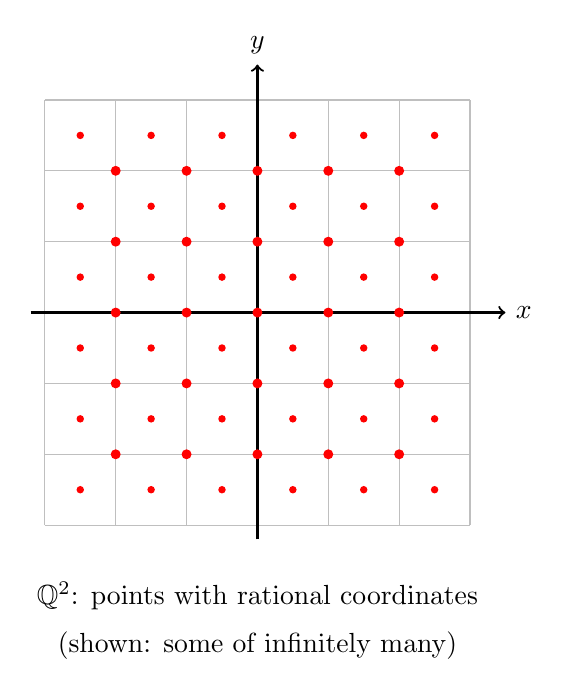
\begin{tikzpicture}[scale=0.9]
    % Grid for R^2
    \draw[gray!50, thin] (-3, -3) grid (3, 3);
    \draw[thick, ->] (-3.2, 0) -- (3.5, 0) node[right] {$x$};
    \draw[thick, ->] (0, -3.2) -- (0, 3.5) node[above] {$y$};

    % Rational points
    \foreach \x in {-2,-1,0,1,2} {
        \foreach \y in {-2,-1,0,1,2} {
            \fill[red] (\x, \y) circle (2pt);
        }
    }

    % Some more rational points
    \foreach \x in {-2.5,-1.5,-0.5,0.5,1.5,2.5} {
        \foreach \y in {-2.5,-1.5,-0.5,0.5,1.5,2.5} {
            \fill[red] (\x, \y) circle (1.5pt);
        }
    }

    \node at (0, -4) {$\Q^2$: points with rational coordinates};
    \node at (0, -4.7) {(shown: some of infinitely many)};
\end{tikzpicture}
\end{center}

\section{Step 1: $\Q^k$ is Countable}

\textbf{Key fact:} Finite products of countable sets are countable.

\begin{center}
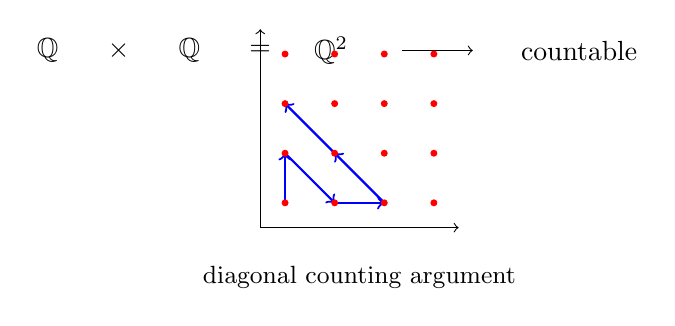
\begin{tikzpicture}[scale=0.9]
    % Show Q x Q
    \node at (-3, 0) {$\Q$};
    \node at (-2, 0) {$\times$};
    \node at (-1, 0) {$\Q$};
    \node at (0, 0) {$=$};
    \node at (1, 0) {$\Q^2$};

    \draw[->] (2, 0) -- (3, 0);
    \node at (4.5, 0) {countable};

    % Visual
    \begin{scope}[yshift=-2.5cm, scale=0.7]
        \draw[->] (0, 0) -- (4, 0);
        \draw[->] (0, 0) -- (0, 4);

        % Diagonal counting
        \draw[blue, thick, ->] (0.5, 0.5) -- (0.5, 1.5);
        \draw[blue, thick, ->] (0.5, 1.5) -- (1.5, 0.5);
        \draw[blue, thick, ->] (1.5, 0.5) -- (2.5, 0.5);
        \draw[blue, thick, ->] (2.5, 0.5) -- (1.5, 1.5);
        \draw[blue, thick, ->] (1.5, 1.5) -- (0.5, 2.5);

        \foreach \x in {0.5, 1.5, 2.5, 3.5} {
            \foreach \y in {0.5, 1.5, 2.5, 3.5} {
                \fill[red] (\x, \y) circle (2pt);
            }
        }

        \node at (2, -1) {\small diagonal counting argument};
    \end{scope}
\end{tikzpicture}
\end{center}

Similarly, $\Q^k = \Q \times \Q \times \cdots \times \Q$ ($k$ times) is countable.

\section{Step 2: $\Q^k$ is Dense in $\R^k$}

We need: every open set in $\R^k$ contains a point of $\Q^k$.

\begin{center}
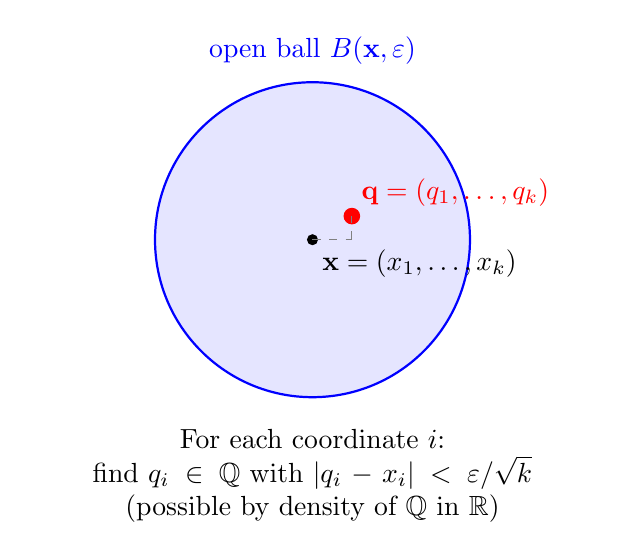
\begin{tikzpicture}[scale=1]
    % An open ball
    \draw[blue, thick, fill=blue!10] (0, 0) circle (2);
    \node[blue] at (0, 2.4) {open ball $B(\mathbf{x}, \varepsilon)$};

    % Center point
    \fill (0, 0) circle (2pt) node[below right] {$\mathbf{x} = (x_1, \ldots, x_k)$};

    % Rational point nearby
    \fill[red] (0.5, 0.3) circle (3pt) node[above right] {$\mathbf{q} = (q_1, \ldots, q_k)$};

    % Show coordinates
    \draw[dashed, gray] (0, 0) -- (0.5, 0);
    \draw[dashed, gray] (0.5, 0) -- (0.5, 0.3);

    \node[text width=7cm, align=center] at (0, -3) {For each coordinate $i$:\\find $q_i \in \Q$ with $|q_i - x_i| < \varepsilon/\sqrt{k}$\\(possible by density of $\Q$ in $\R$)};
\end{tikzpicture}
\end{center}

\textbf{Why does this work?}

\begin{align*}
|\mathbf{q} - \mathbf{x}| &= \sqrt{\sum_{i=1}^{k} (q_i - x_i)^2} \\
&< \sqrt{\sum_{i=1}^{k} \left(\frac{\varepsilon}{\sqrt{k}}\right)^2} \\
&= \sqrt{k \cdot \frac{\varepsilon^2}{k}} = \varepsilon
\end{align*}

So $\mathbf{q} \in B(\mathbf{x}, \varepsilon)$. Done!

\section{Visual Summary}

\begin{center}
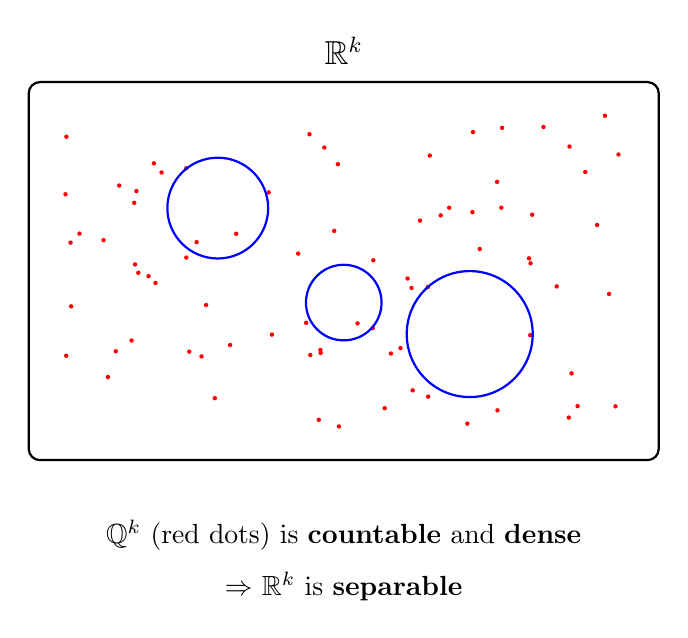
\begin{tikzpicture}[scale=0.8]
    % Big picture
    \draw[thick, rounded corners] (-5, -3) rectangle (5, 3);
    \node at (0, 3.5) {\large $\R^k$};

    % Q^k as a dense subset
    \foreach \i in {1,...,80} {
        \pgfmathsetmacro{\x}{-4.5 + 9*rnd}
        \pgfmathsetmacro{\y}{-2.5 + 5*rnd}
        \fill[red] (\x, \y) circle (1pt);
    }

    % Some open sets
    \draw[blue, thick] (-2, 1) circle (0.8);
    \draw[blue, thick] (2, -1) circle (1);
    \draw[blue, thick] (0, -0.5) circle (0.6);

    \node at (0, -4.2) {$\Q^k$ (red dots) is \textbf{countable} and \textbf{dense}};
    \node at (0, -5) {$\Rightarrow$ $\R^k$ is \textbf{separable}};
\end{tikzpicture}
\end{center}

\section{Why Does This Matter?}

Separability is important because:
\begin{itemize}
    \item It means the space isn't ``too big'' — it can be approximated by a countable set
    \item Separable spaces have countable bases (see Rudin 2.23)
    \item Many theorems in analysis require separability
\end{itemize}

\end{document}
